\documentclass[letterpaper,12pt,fleqn]{article}
\usepackage{matharticle}
\usepackage{mathtools}
\usepackage{tikz}
\usepackage{graphicx}
\renewcommand{\o}{\theta}
\pagestyle{plain}
\begin{document}

\begin{center}
\Large Math-19 Homework \#8 Solutions
\end{center}

\vspace{0.5in}

\underline{Reading}

Please read sections 5.4-5.6 and 6.4-6.6, then do all concept problems in the
posted sections on web\-assign.

\underline{Problems}

\begin{enumerate}
\item Consider the function:
\[f(x)=2\tan(4\pi x-\pi)+1=2\tan4\pi\left(x-\frac{1}{4}\right)+1\]
\begin{enumerate}
\item What is the period $P$?
  \[P=\frac{\pi}{4\pi}=\frac{1}{4}\]
  
\item What is the horizontal translation $b$?
  \[\frac{1}{4}\ \mbox{to the right}\]
  
\item What is the phase angle $\phi$?
  \[\pi=-\pi\]

\item What is the y-intercept?
  \[f(0)=2\tan(-\pi)+1=0+1=1\]
  
\item Sketch one cycle of the graph in the interval $(b,b+P)$ and then extend
  the sketch back to the y-intercept.
  
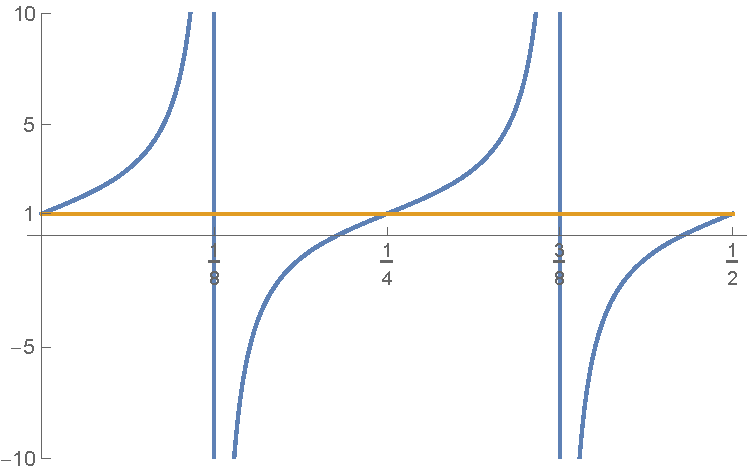
\includegraphics{tan}
\end{enumerate}

\item Solve for $x$:
\[\tan\left(3x+\frac{\pi}{2}\right)\sin(2\pi x)\cos(6x+\pi)=0\]
Hint: be careful about domain!

Each of the factors results in a set of solutions:

\begin{eqnarray*}
  \tan\left(3x+\frac{\pi}{2}\right) &=& 0 \\
  3x+\frac{\pi}{2} &=& k\pi \\
  3x &=& -\frac{\pi}{2}+k\pi \\
  x &=& -\frac{\pi}{6}+k\frac{\pi}{3} \\
\end{eqnarray*}
\begin{eqnarray*}
  \sin(2\pi x) &=& 0 \\
  2\pi x &=& k\pi \\
  x &=& \frac{k}{2} \\
\end{eqnarray*}
\begin{eqnarray*}
  \cos(6x+\pi) &=& 0 \\
  6x+\pi &=& \frac{\pi}{2}+k\pi \\
  6x &=& -\frac{\pi}{2}+k\pi \\
  x &=& -\frac{\pi}{12}+k\frac{\pi}{6} \\
\end{eqnarray*}

As a final check, we make sure that none of the solutions violate the domain
of the tangent function. Since none of the solutions to the sine or cosine
parts land on a vertical asymptote, all of the solutions are OK.

\bigskip

\item Two $1kg$ masses are each suspended on a spring with $k=\pi^2$ and are
stretched downward by 2 units. The first spring is released at $t=0$. The
second spring is released at $t=3$.
\begin{enumerate}
\item Find $f_1(t)$ for the first mass.
  \[f_1(t)=2\cos\left(\sqrt{\frac{\pi^2}{1}}t\right)=2\cos\pi t\]
  
\item Find $f_2(t)$ for the second mass.
  \[f_2(t)=2\cos\pi(t-3)=2\cos(\pi t-3\pi)\]

\item What is the phase difference between the two masses?

  The phase angle in the previous part is $3\pi$; however, since the period is
  only $2\pi$, we can state the phase angle as $3\pi-2\pi=\pi$ or $180^{\circ}$.
\end{enumerate}

\bigskip

\item Evaluate:
  \[\cot\left(\cos^{-1}\frac{x}{\sqrt{1+x^2}}\right)\]

  First, we repeat to ourselves, ``the angle whose cosine is ....'' Next, we
  draw a right triangle corresponding to our angle:

  \begin{figure}[h]
  \setlength{\leftskip}{1in}
  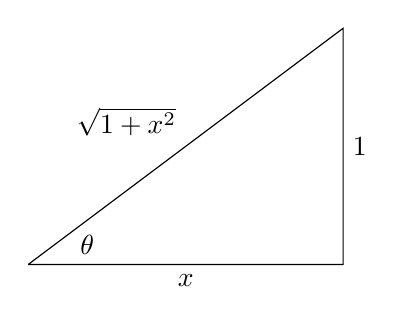
\begin{tikzpicture}
    \draw (0,0) -- (4,0) -- (4,3) -- (0,0);
    \node at (0.75,0.25) {$\o$};
    \node [below] at (2,0) {$x$};
    \node [right] at (4,1.5) {$1$};
    \node [above left] at (2,1.5) {$\sqrt{1+x^2}$};
  \end{tikzpicture}
  \end{figure}

  Note that by using the Pythagorean theorem we determine that the length of
  the opposite side is 1.  We now take the cotangent of our angle:
  \[\cot\left(\cos^{-1}\frac{x}{\sqrt{1+x^2}}\right)=\frac{x}{1}=x\]

\item Consider the following triangle:

\bigskip

\begin{figure}[h]
\setlength{\leftskip}{0.5in}
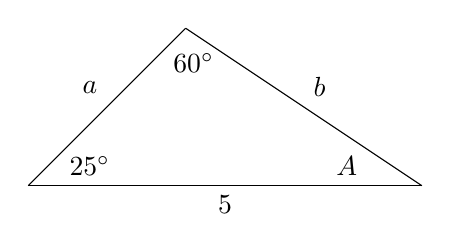
\begin{tikzpicture}
\draw (0,0) -- (5,0);
\draw (0,0) -- (2,2);
\draw (5,0) -- (2,2);
\node [below] at (2.5,0) {$5$};
\node [left] at (1,1.25) {$a$};
\node [right] at (3.5,1.25) {$b$};
\node [below] at (2.1,1.8) {$60^{\circ}$};
\node [above right] at (0.4,0) {$25^{\circ}$};
\node [above left] at (4.3,0) {$A$};
\end{tikzpicture}
\end{figure}

\begin{enumerate}
\item Determine $A$.
  \[A=180^{\circ}-(60^{\circ}+25^{\circ})=180^{\circ}-85^{\circ}=95^{\circ}\]
  
\item Determine $a$.
  \[\frac{\sin{95^{\circ}}}{a}=\frac{\sin{60^{\circ}}}{5}\]
  \[a=\frac{5\sin{95^{\circ}}}{\sin{60^{\circ}}}\]
  \[a=5.75\]
    
\item Determine $b$.
  \[\frac{\sin{25^{\circ}}}{b}=\frac{\sin{60^{\circ}}}{5}\]
  \[b=\frac{5\sin{25^{\circ}}}{\sin{60^{\circ}}}\]
  \[b=2.44\]

\item Using Heron's Formula, determine the area of the triangle.
  \[s=\frac{5+5.75+2.44}{2}=6.6\]
  \[A=\sqrt{6.6(6.6-5)(6.6-5.75)(6.6-2.44)}=6.11\]
\end{enumerate}
\end{enumerate}
\end{document}
